\chapter{Conclusions and Future Work}\label{chp:chp7}

%\begin{flushright}
%  {\em QUOTE GOES HERE }\\
%
%\ \
%
%\normalsize
%{AUTHOR}  
%\end{flushright}


\noindent{In this thesis I have attempted to elucidate the potential contribution that CCSNe make to the formation of dust in the universe.  I have written, developed and tested a new Monte Carlo code, {\sc damocles}, and I have used it to model line profiles  from a number of SNRs that exhibit the characteristic red-blue asymmetry that indicates the presence of dust in SNR ejecta.  In these final few pages, I will summarise the key results that I have presented and I will consider the potential for developments to the code and work in the future.}

\section{Signatures of Dust Formation in Characteristic Line Profiles}

I have been interested in modelling dust in the ejecta of CCSNe.  In particular, this has necessitated the parametrisation of the expanding debris of a CCSN via a number of properties.  Specifically, the ejecta has generally been defined by the following quantities:

\begin{itemize}
\item the maximum velocity, $V_{max}$
\item the ejecta radius ratio, $R_{in}/R_{out}$
\item the dust optical depth,  $\tau$
\item the dust albedo, $\omega$ 
\item the dust and gas density profile exponent, $\beta$, where $\rho \propto r^{-\beta}$
\end{itemize}

The effects of varying each of these parameters were discussed in detail in Chapter \ref{chp:chp4} but there are a few key results that I will mention here.  Traditionally, the blue-shifted nature of line profiles from the ejecta of supernovae has been thought to arise from high dust optical depths causing the entire profile to become shifted towards the blue.  This has resulted in an expectation that the position of the peaks of blue-shifted line profiles observed in a single spectrum will be wavelength dependent, with wavelengths that undergo greater attenuation by dust grains experiencing stronger blue-shifting than those that are less affected.  In practice, this has rarely been seen and occasionally this is used as an argument against dust being the cause of observed asymmetries.  My models of theoretical line profiles have suggested that, whilst this can be the case, it is also possible that the line profiles can exhibit a blue-shifted peak simply as a result of an intrinsically flat-topped profile that suffers attenuation on the red side leaving the peak flux at the value of the minimum velocity on the blue side.  In this case, the velocities of the peak fluxes of line profiles in a spectrum are not wavelength dependent but rather trace the location of the emitting ions in the ejecta.

\begin{figure}
\centering
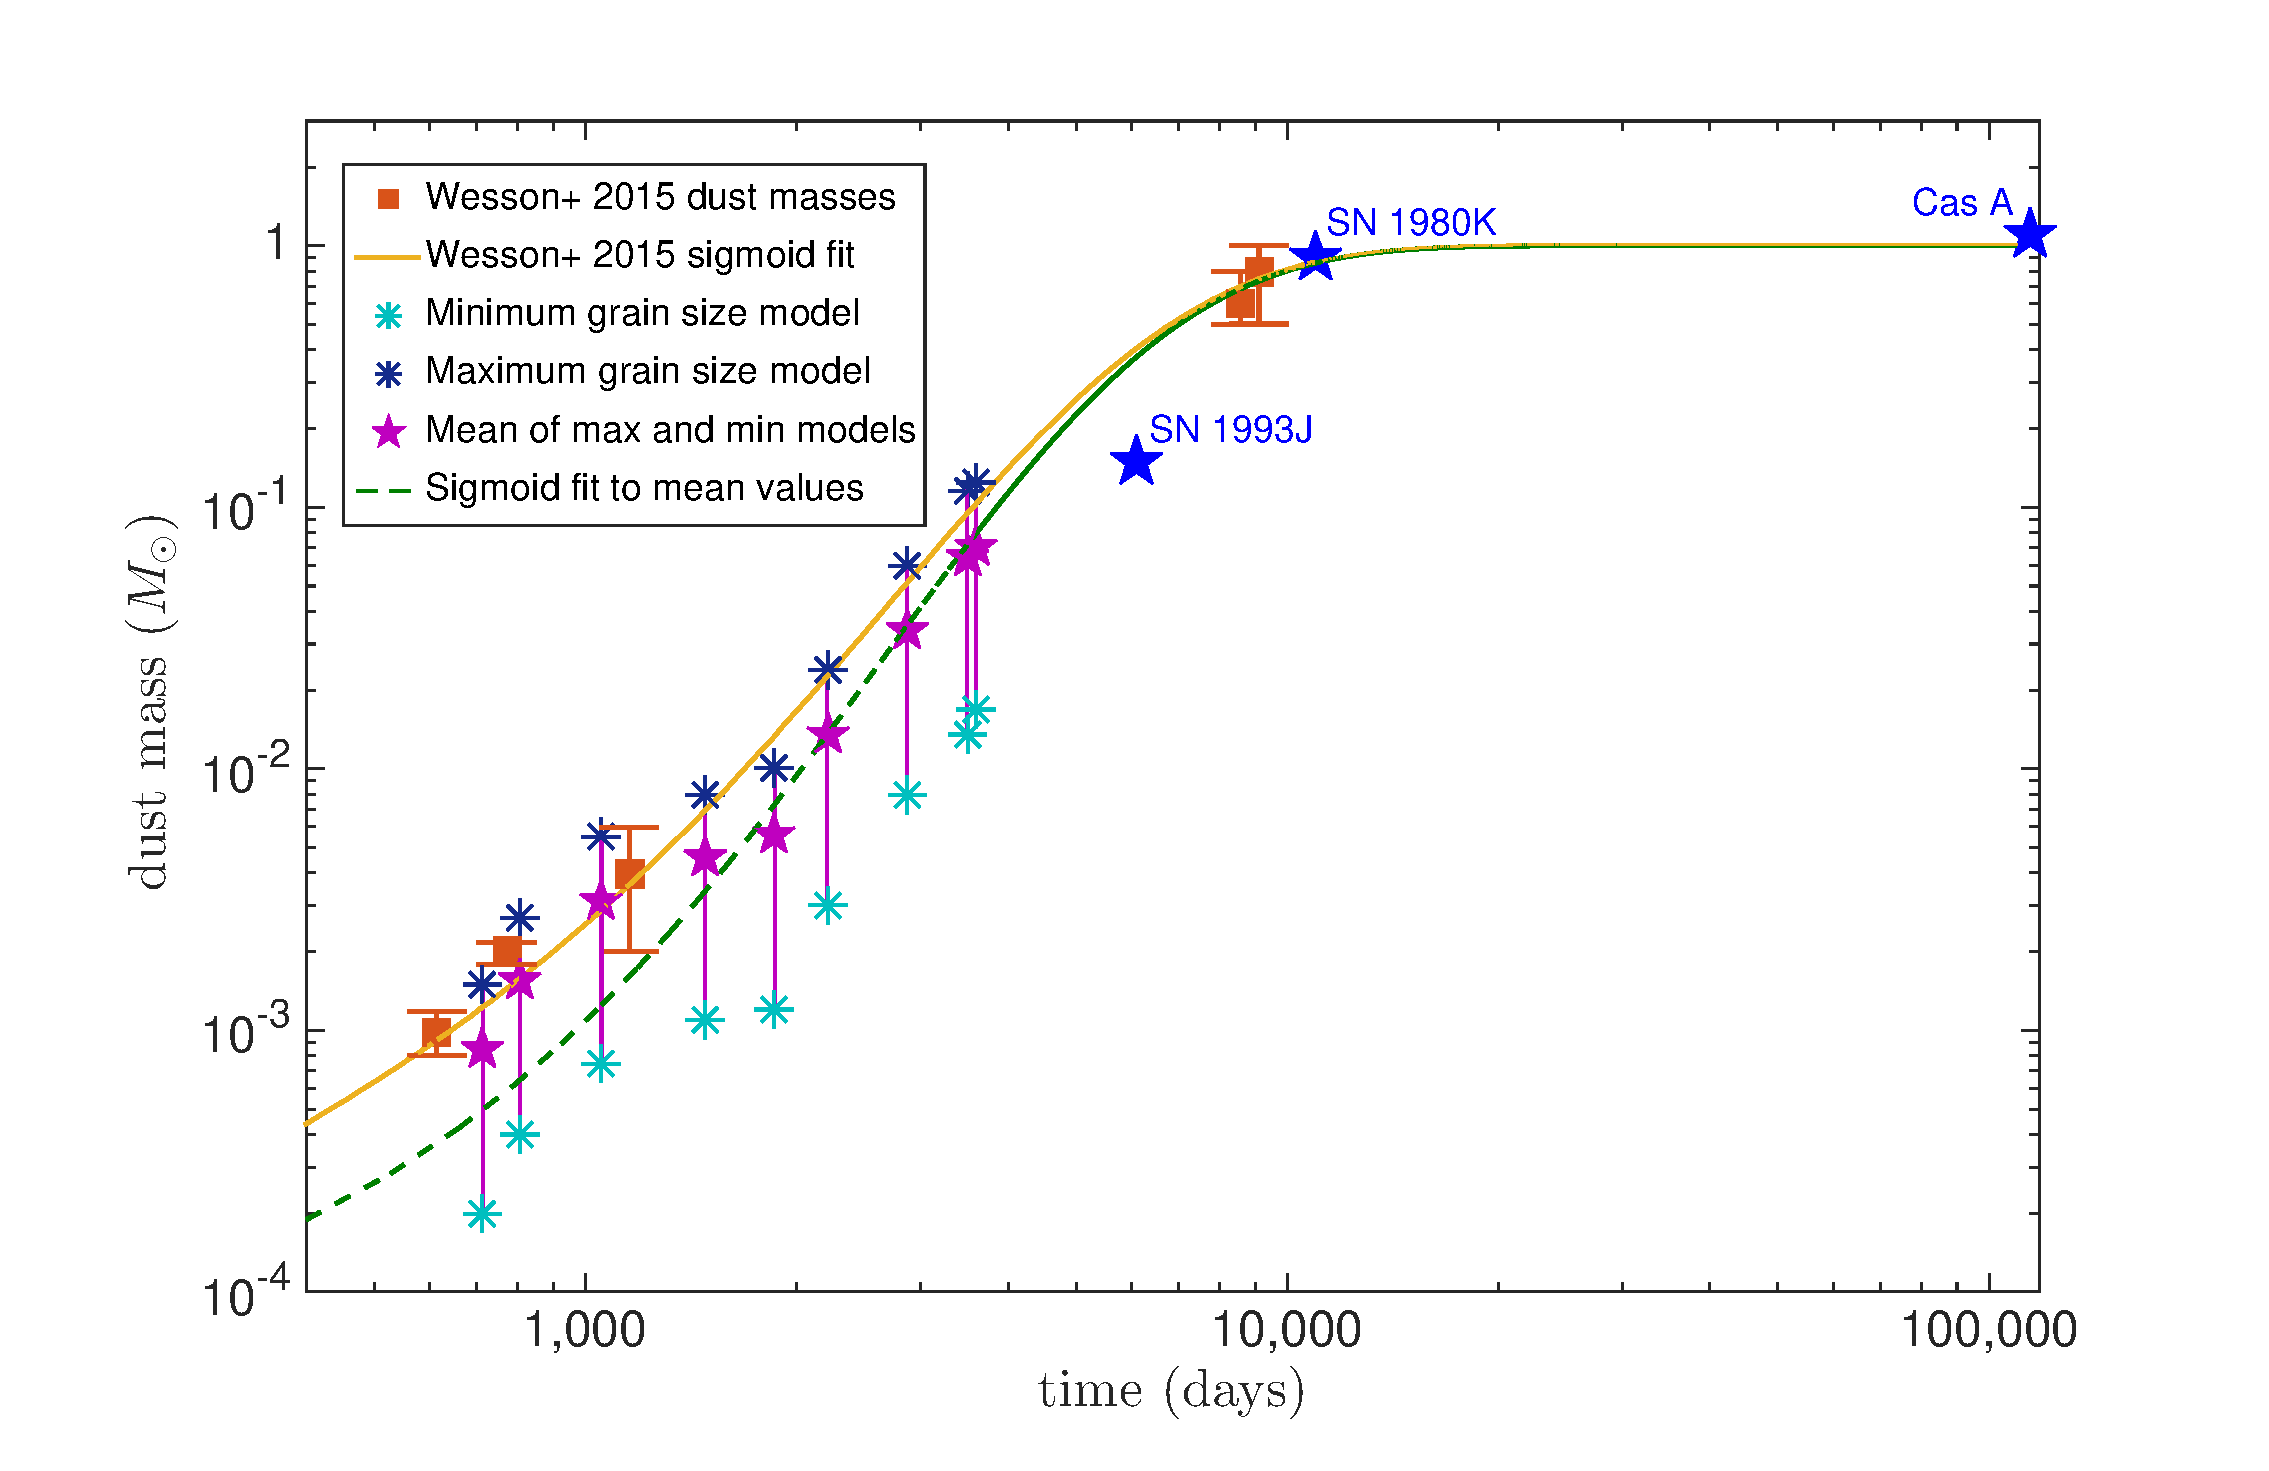
\includegraphics[scale=0.43,clip=true, trim=45 15 80 30]{chapters/chapter7/figs/Mdust_evol9.eps}
\caption{Dust masses for SN~1987A, SN~1980K, SN~1993J and Cas~A. \textit{Red squares -} SN~1987A dust masses derived by W15. \textit{Yellow line} - 
W15's sigmoid fit to 
their values. \textit{Dark and light blue asterisks -} maximum 
($a=3.5~\mu$m) and 
minimum ($a=0.6~\mu$m) SN~1987A dust masses respectively for the [O~{\sc i}] models 
for $t \le 1478$ days and for the H$\alpha$ models for $t \ge 1862$ days. 
\textit{Purple 
stars -}  the mean of the maximum and 
minimum SN~1987A dust masses.
\textit{Green line -} sigmoid fit 
to the SN~1987A mean dust masses.  \textit{Blue stars -} dust masses derived from the year 31 amorphous carbon model for the SN~1980K [O~{\sc i}] doublet, the year 16 silicate model for the SN~1993J  [O~{\sc iii}] doublet and the mixed composition model for the Cas~A [O~{\sc iii}] doublet with 50\% amorphous carbon grains and 50\% silicate grains.}
\label{dust1}
\end{figure}

Similarly, there is a general expectation that dust-affected line profiles exhibit a flux bias towards the blue.  In fact, the theoretical profiles presented in Chapter \ref{chp:chp4} suggest that in cases of extremely scattering dusty nebulae, the effects of absorption are decreased relative to the effects of scattering and the overall flux bias of the profile is in fact towards the red.  This requires relatively extreme conditions and will likely not be a common occurrence however.   Regardless of the flux bias, the peak must always be either central or blue-shifted and cannot be shifted to the red via dust extinction effects.  

The effects of dust scattering also frequently result in a red scattering wing that extends well beyond the theoretical maximum velocity.  This feature, that was noted by \citet{Lucy1989} and that I discussed based on my theoretical investigation of parameter space, was seen in several of the line profiles that I presented throughout this thesis for different supernovae.  The presence of this extended red scattering wing in observed line profiles allowed me to place constraints on the albedo and hence the dust grain radius for a given species.  The potential for double-peaked profiles with a red-shifted trough between the peak fluxes at $+V_{min}$ and $-V_{min}$ is also noted as a potential signature for dust in the ejecta.

\section{Dust Masses in Core-Collapse Supernovae}

In Chapters \ref{chp:chp5} and \ref{chp:chp6} I presented models for the hydrogen and oxygen line profiles of four different SNRs and I obtained dust masses based on these models.  Whilst I have discussed these findings in context for each of these supernovae, it is useful here to place these dust masses into the wider context of the dust masses deduced for a range of CCSNe at different epochs.  

\begin{figure}
\centering
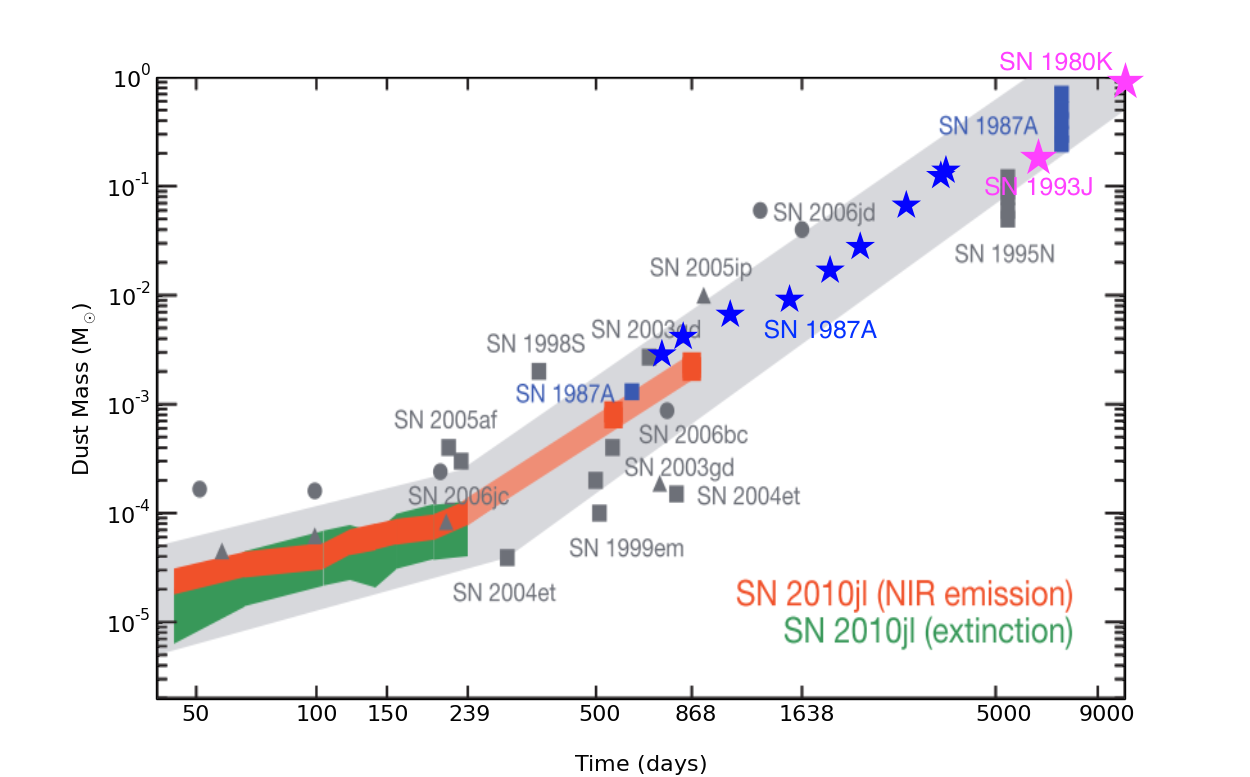
\includegraphics[scale=0.55,clip=true, trim=50 0 60 30]{chapters/chapter7/figs/final_dust_plot2.png}
\caption{Dust formation rate in CCSNe as taken from the study of SN~2010jl by \citet{Gall2014}.  Over-plotted in purple stars are the dust masses derived from the amorphous carbon model of the [O~{\sc i}] doublet for SN~1980K and the silicate model of the [O~{\sc iii}] doublet for SN~1993J.  The blue stars are the maximum dust masses derived from my amorphous carbon models of the H$\alpha$ and [O~{\sc i}]$\lambda\lambda$6300,6363~\AA\ lines as presented in Figure \ref{Mdust}.}
\label{dust2}
\end{figure}

I have already discussed the findings of \citet{Wesson2015} in Section \ref{discuss} and compared the rate of dust formation in SN~1987A indicated by my models with the rate of dust formation that they derived.  It is useful to consider how the dust masses that I obtained in the previous chapter for SN~1980K and SN~1993J compare to these results.  In Figure \ref{dust1}, I include a plot illustrating the dust masses derived for SN~1987A from SED fitting and from my line profile modelling and I add to this plot the dust masses that I obtained for SN~1993J, SN~1980K and Cas~A.  As can be seen, these results are in reasonable agreement and suggest that large masses of dust have indeed formed by late epochs decades after outburst.  The dust mass derived for SN~1993J at 16 years after outburst is somewhat lower than might be predicted based on the dust mass evolution of SN~1987A at a similar epoch but this may be because of different conditions in the ejecta corresponding to their different spectral classifications (SN~1993J was a Type IIb supernova whereas SN~1987A and SN~1980K were more common Type IIP and Type IIL supernovae respectively).

In their analyses of photometric and spectroscopic observations of SN~2010jl, \citet{Gall2014} presented a plot of the expected rate of dust formation in the ejecta of CCSNe and included on their plot a number of dust mass estimates for different objects at different epochs.  I include this plot in Figure \ref{dust2} and superimpose on it the dust mass estimates that I obtain for SN~1987A across the full range of epochs that I modelled. I also include the dust mass estimates for SN~1993J and SN~1980K at 16~years and 31~years after outburst respectively.  The results agree strongly with the dust formation rates plotted  by \citet{Gall2014}.

Even accounting for difficulties in determining dust grain sizes and the dust composition, the dust masses that I derive for all profiles consistently suggest that large masses of dust of the order of $\sim0.1-0.9$~M$_{\odot}$ are required in order to reproduce the asymmetries observed in  line profiles from the ejecta of CCSNe at late times.  
%Careful consideration should also be paid to the fraction of dust that is capable of surviving the passage of the reverse shock when contemplating CCSNe as the solution to the dust budget problem in the early universe. 

\section{Potential Future Work}

The {\sc damocles} code has the potential to be developed in a number of ways in the future in order to improve its capacity to constrain dust masses in the ejecta of CCSNe.  Currently, Mie theory is employed to treat dust grains as spherical particles when in practice dust grains are likely a variety of shapes.  Extension of the code to treat different grain morphologies by including a continuous distribution of ellipsoids or replacing the Mie theory routine with alternatives such as the Discrete Dipole Approximation or the T-Matrix Method would address this limitation. The code could also be extended to include the capacity to treat polarised radiation.  This would allow models not only to reproduce line profiles but also to reproduce the polarisation of the observed packets across the wavelength range of interest.  One of the current assumptions for these models is that the emitted lines are optically thin.  It is possible that there will be scenarios, particularly at earlier epochs, where this is not the case.  By including the Sobolev approximation \citep{Sobolev1957} in the code, this issue could be largely resolved.  Finally, manual investigation of parameter space, whilst it has a number of advantages, can also be laborious and time consuming.  The application of an MCMC methodology to investigate parameter space in an automated fashion in order to produce probability density functions for each parameter and to better understand the interdependence of the parameters of interest would allow for increasingly higher dimensional parameter spaces to be explored effectively.

More generally, further ejecta models that include more complex geometries and use  more representative dust  compositions should be produced in order to further constrain the dust masses forming in these objects. Models of more blue-shifted lines from other CCSNe observed at late times will help to further clarify the picture of dust formation in CCSNe.

%General features of profiles
%-red scat wing
%-absorption not necessarily blue flux biased
%-peak may be central or blue-shifted
%-double peaked emission lines may be seen due to absorption in central regions, but trough will be red-shifted
%
%General limitations of modelling asymmetric line profiles
%-complex/asymmetric geometries have significant effect on line profiles
%-noisy
%-most effective when can limit based on red wing, but still dependent on species
% 
%Broad results
%-nonetheless obtain strong results that are broadly in agreement with SED fitting
%-got evolution of SN~1987A in strong agreement with Gall 2014
%-also got large masses at late times
%-then the dust plot
%-then wrap up lots of dust in sne and relate back to dust budget proble in the early universe - remind them what the point was!

